\PassOptionsToPackage{unicode=true}{hyperref} % options for packages loaded elsewhere
\PassOptionsToPackage{hyphens}{url}
%
\documentclass[]{article}
\usepackage{lmodern}
\usepackage{amssymb,amsmath}
\usepackage{ifxetex,ifluatex}
\usepackage{fixltx2e} % provides \textsubscript
\ifnum 0\ifxetex 1\fi\ifluatex 1\fi=0 % if pdftex
  \usepackage[T1]{fontenc}
  \usepackage[utf8]{inputenc}
  \usepackage{textcomp} % provides euro and other symbols
\else % if luatex or xelatex
  \usepackage{unicode-math}
  \defaultfontfeatures{Ligatures=TeX,Scale=MatchLowercase}
\fi
% use upquote if available, for straight quotes in verbatim environments
\IfFileExists{upquote.sty}{\usepackage{upquote}}{}
% use microtype if available
\IfFileExists{microtype.sty}{%
\usepackage[]{microtype}
\UseMicrotypeSet[protrusion]{basicmath} % disable protrusion for tt fonts
}{}
\IfFileExists{parskip.sty}{%
\usepackage{parskip}
}{% else
\setlength{\parindent}{0pt}
\setlength{\parskip}{6pt plus 2pt minus 1pt}
}
\usepackage{hyperref}
\hypersetup{
            pdftitle={Visualization Examples},
            pdfauthor={SDS 291},
            pdfborder={0 0 0},
            breaklinks=true}
\urlstyle{same}  % don't use monospace font for urls
\usepackage[margin=1in]{geometry}
\usepackage{color}
\usepackage{fancyvrb}
\newcommand{\VerbBar}{|}
\newcommand{\VERB}{\Verb[commandchars=\\\{\}]}
\DefineVerbatimEnvironment{Highlighting}{Verbatim}{commandchars=\\\{\}}
% Add ',fontsize=\small' for more characters per line
\usepackage{framed}
\definecolor{shadecolor}{RGB}{248,248,248}
\newenvironment{Shaded}{\begin{snugshade}}{\end{snugshade}}
\newcommand{\AlertTok}[1]{\textcolor[rgb]{0.94,0.16,0.16}{#1}}
\newcommand{\AnnotationTok}[1]{\textcolor[rgb]{0.56,0.35,0.01}{\textbf{\textit{#1}}}}
\newcommand{\AttributeTok}[1]{\textcolor[rgb]{0.77,0.63,0.00}{#1}}
\newcommand{\BaseNTok}[1]{\textcolor[rgb]{0.00,0.00,0.81}{#1}}
\newcommand{\BuiltInTok}[1]{#1}
\newcommand{\CharTok}[1]{\textcolor[rgb]{0.31,0.60,0.02}{#1}}
\newcommand{\CommentTok}[1]{\textcolor[rgb]{0.56,0.35,0.01}{\textit{#1}}}
\newcommand{\CommentVarTok}[1]{\textcolor[rgb]{0.56,0.35,0.01}{\textbf{\textit{#1}}}}
\newcommand{\ConstantTok}[1]{\textcolor[rgb]{0.00,0.00,0.00}{#1}}
\newcommand{\ControlFlowTok}[1]{\textcolor[rgb]{0.13,0.29,0.53}{\textbf{#1}}}
\newcommand{\DataTypeTok}[1]{\textcolor[rgb]{0.13,0.29,0.53}{#1}}
\newcommand{\DecValTok}[1]{\textcolor[rgb]{0.00,0.00,0.81}{#1}}
\newcommand{\DocumentationTok}[1]{\textcolor[rgb]{0.56,0.35,0.01}{\textbf{\textit{#1}}}}
\newcommand{\ErrorTok}[1]{\textcolor[rgb]{0.64,0.00,0.00}{\textbf{#1}}}
\newcommand{\ExtensionTok}[1]{#1}
\newcommand{\FloatTok}[1]{\textcolor[rgb]{0.00,0.00,0.81}{#1}}
\newcommand{\FunctionTok}[1]{\textcolor[rgb]{0.00,0.00,0.00}{#1}}
\newcommand{\ImportTok}[1]{#1}
\newcommand{\InformationTok}[1]{\textcolor[rgb]{0.56,0.35,0.01}{\textbf{\textit{#1}}}}
\newcommand{\KeywordTok}[1]{\textcolor[rgb]{0.13,0.29,0.53}{\textbf{#1}}}
\newcommand{\NormalTok}[1]{#1}
\newcommand{\OperatorTok}[1]{\textcolor[rgb]{0.81,0.36,0.00}{\textbf{#1}}}
\newcommand{\OtherTok}[1]{\textcolor[rgb]{0.56,0.35,0.01}{#1}}
\newcommand{\PreprocessorTok}[1]{\textcolor[rgb]{0.56,0.35,0.01}{\textit{#1}}}
\newcommand{\RegionMarkerTok}[1]{#1}
\newcommand{\SpecialCharTok}[1]{\textcolor[rgb]{0.00,0.00,0.00}{#1}}
\newcommand{\SpecialStringTok}[1]{\textcolor[rgb]{0.31,0.60,0.02}{#1}}
\newcommand{\StringTok}[1]{\textcolor[rgb]{0.31,0.60,0.02}{#1}}
\newcommand{\VariableTok}[1]{\textcolor[rgb]{0.00,0.00,0.00}{#1}}
\newcommand{\VerbatimStringTok}[1]{\textcolor[rgb]{0.31,0.60,0.02}{#1}}
\newcommand{\WarningTok}[1]{\textcolor[rgb]{0.56,0.35,0.01}{\textbf{\textit{#1}}}}
\usepackage{graphicx,grffile}
\makeatletter
\def\maxwidth{\ifdim\Gin@nat@width>\linewidth\linewidth\else\Gin@nat@width\fi}
\def\maxheight{\ifdim\Gin@nat@height>\textheight\textheight\else\Gin@nat@height\fi}
\makeatother
% Scale images if necessary, so that they will not overflow the page
% margins by default, and it is still possible to overwrite the defaults
% using explicit options in \includegraphics[width, height, ...]{}
\setkeys{Gin}{width=\maxwidth,height=\maxheight,keepaspectratio}
\setlength{\emergencystretch}{3em}  % prevent overfull lines
\providecommand{\tightlist}{%
  \setlength{\itemsep}{0pt}\setlength{\parskip}{0pt}}
\setcounter{secnumdepth}{0}
% Redefines (sub)paragraphs to behave more like sections
\ifx\paragraph\undefined\else
\let\oldparagraph\paragraph
\renewcommand{\paragraph}[1]{\oldparagraph{#1}\mbox{}}
\fi
\ifx\subparagraph\undefined\else
\let\oldsubparagraph\subparagraph
\renewcommand{\subparagraph}[1]{\oldsubparagraph{#1}\mbox{}}
\fi

% set default figure placement to htbp
\makeatletter
\def\fps@figure{htbp}
\makeatother


\title{Visualization Examples}
\author{SDS 291}
\date{4/20/2020}

\begin{document}
\maketitle

{
\setcounter{tocdepth}{2}
\tableofcontents
}
\hypertarget{visualizing-distributions-frequencies}{%
\section{Visualizing Distributions \&
Frequencies}\label{visualizing-distributions-frequencies}}

You likely want to offer your reader or poster viewer some descriptive
statistics or sense of the distribution/frequency of your variables of
interest.

\begin{Shaded}
\begin{Highlighting}[]
\KeywordTok{library}\NormalTok{(Stat2Data)}
\KeywordTok{data}\NormalTok{(}\StringTok{"Titanic"}\NormalTok{)}
\NormalTok{newTitanic <-}\StringTok{ }\NormalTok{Titanic }\OperatorTok\StringTok{ }\KeywordTok{filter}\NormalTok{(PClass }\OperatorTok{!=}\StringTok{ "*"}\NormalTok{) }\OperatorTok\StringTok{ }\KeywordTok{mutate}\NormalTok{(}\DataTypeTok{Survived2 =} \KeywordTok{as.factor}\NormalTok{(}\KeywordTok{if_else}\NormalTok{(Survived }\OperatorTok{==}\StringTok{ }
\StringTok{    }\DecValTok{1}\NormalTok{, }\StringTok{"Yes"}\NormalTok{, }\KeywordTok{if_else}\NormalTok{(Survived }\OperatorTok{==}\StringTok{ }\DecValTok{0}\NormalTok{, }\StringTok{"No"}\NormalTok{, }\OtherTok{NA_character_}\NormalTok{))))}
\end{Highlighting}
\end{Shaded}

\hypertarget{binary-response-variable-quantitative-explanatory-variable}{%
\subsection{Binary Response Variable, Quantitative Explanatory
Variable}\label{binary-response-variable-quantitative-explanatory-variable}}

\hypertarget{boxplot}{%
\subsubsection{Boxplot}\label{boxplot}}

You might want to illustrate the same kind of boxplot we've seen for
logistic regression \emph{by} some other variable -- probably a variable
you plan as an interaction hypothesis.

\begin{Shaded}
\begin{Highlighting}[]
\NormalTok{Survival_Age_Box <-}\StringTok{ }\NormalTok{newTitanic }\OperatorTok\StringTok{ }\KeywordTok{ggplot}\NormalTok{(}\KeywordTok{aes}\NormalTok{(}\DataTypeTok{y =}\NormalTok{ Age, }\DataTypeTok{x =}\NormalTok{ Survived2, }
    \DataTypeTok{fill =}\NormalTok{ Sex)) }\OperatorTok{+}\StringTok{ }\CommentTok{# Making Thicker Lines for the Boxplot}
\KeywordTok{geom_boxplot}\NormalTok{(}\DataTypeTok{position =} \KeywordTok{position_dodge}\NormalTok{(}\FloatTok{0.9}\NormalTok{), }\DataTypeTok{lwd =} \FloatTok{1.2}\NormalTok{) }\OperatorTok{+}\StringTok{ }\KeywordTok{coord_flip}\NormalTok{() }\OperatorTok{+}\StringTok{ }
\StringTok{    }\KeywordTok{theme_bw}\NormalTok{() }\OperatorTok{+}\StringTok{ }\KeywordTok{labs}\NormalTok{(}\DataTypeTok{y =} \StringTok{"Age"}\NormalTok{, }\DataTypeTok{x =} \StringTok{"Survived"}\NormalTok{, }\DataTypeTok{title =} \StringTok{"Distribution of Age of Titanic Passengers }\CharTok{\textbackslash{}n}\StringTok{by Survival and Sex"}\NormalTok{) }\OperatorTok{+}\StringTok{ }
\StringTok{    }\CommentTok{# Making the font big so it's easy to see on a poster}
\KeywordTok{theme}\NormalTok{(}\DataTypeTok{legend.position =} \StringTok{"bottom"}\NormalTok{, }\DataTypeTok{text =} \KeywordTok{element_text}\NormalTok{(}\DataTypeTok{size =} \DecValTok{20}\NormalTok{))}

\NormalTok{Survival_Age_Box}
\end{Highlighting}
\end{Shaded}

\begin{verbatim}
## Warning: Removed 556 rows containing non-finite values (stat_boxplot).
\end{verbatim}

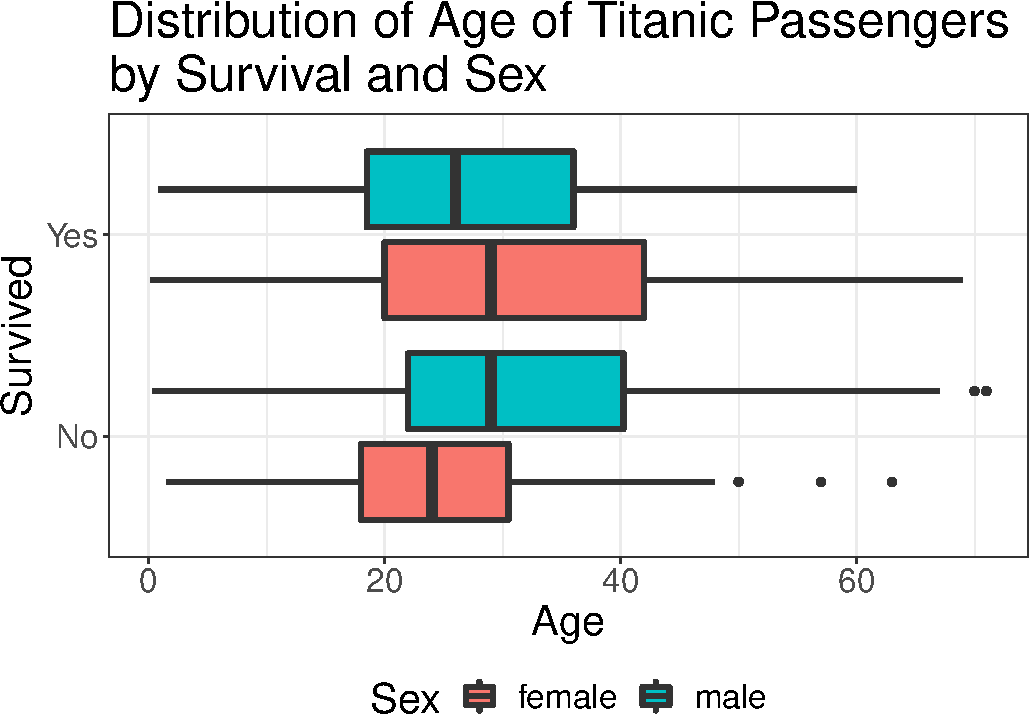
\includegraphics{Visualization_Examples_2020_v01_files/figure-latex/unnamed-chunk-2-1.pdf}

\hypertarget{distributions}{%
\subsubsection{Distributions}\label{distributions}}

You could also use a ridge plot from \texttt{ggridges} package (you
might need to install it) to show the same pattern as a smoothed
distribution, like a density plot, that shows not just the median and
quantiles like a boxplot does.

\begin{Shaded}
\begin{Highlighting}[]
\KeywordTok{library}\NormalTok{(ggridges)}
\NormalTok{Survival_Age_Ridges <-}\StringTok{ }\NormalTok{newTitanic }\OperatorTok\StringTok{ }\KeywordTok{ggplot}\NormalTok{(}\KeywordTok{aes}\NormalTok{(}\DataTypeTok{y =}\NormalTok{ Survived2)) }\OperatorTok{+}\StringTok{ }
\StringTok{    }\KeywordTok{geom_density_ridges}\NormalTok{(}\KeywordTok{aes}\NormalTok{(}\DataTypeTok{x =}\NormalTok{ Age, }\DataTypeTok{fill =}\NormalTok{ Sex), }\DataTypeTok{alpha =} \FloatTok{0.8}\NormalTok{, }\DataTypeTok{color =} \StringTok{"white"}\NormalTok{, }
        \DataTypeTok{from =} \DecValTok{0}\NormalTok{, }\DataTypeTok{to =} \DecValTok{100}\NormalTok{) }\OperatorTok{+}\StringTok{ }\KeywordTok{labs}\NormalTok{(}\DataTypeTok{x =} \StringTok{"Age"}\NormalTok{, }\DataTypeTok{y =} \StringTok{"Survival"}\NormalTok{, }\DataTypeTok{title =} \StringTok{"Distribution of Age of Titanic Passengers }\CharTok{\textbackslash{}n}\StringTok{by Survival and Sex"}\NormalTok{) }\OperatorTok{+}\StringTok{ }
\StringTok{    }\KeywordTok{scale_y_discrete}\NormalTok{(}\DataTypeTok{expand =} \KeywordTok{c}\NormalTok{(}\FloatTok{0.01}\NormalTok{, }\DecValTok{0}\NormalTok{)) }\OperatorTok{+}\StringTok{ }\KeywordTok{scale_x_continuous}\NormalTok{(}\DataTypeTok{expand =} \KeywordTok{c}\NormalTok{(}\FloatTok{0.01}\NormalTok{, }
    \DecValTok{0}\NormalTok{)) }\OperatorTok{+}\StringTok{ }\KeywordTok{theme_ridges}\NormalTok{(}\DataTypeTok{grid =} \OtherTok{FALSE}\NormalTok{) }\OperatorTok{+}\StringTok{ }\KeywordTok{theme}\NormalTok{(}\DataTypeTok{legend.position =} \StringTok{"bottom"}\NormalTok{)}

\NormalTok{Survival_Age_Ridges}
\end{Highlighting}
\end{Shaded}

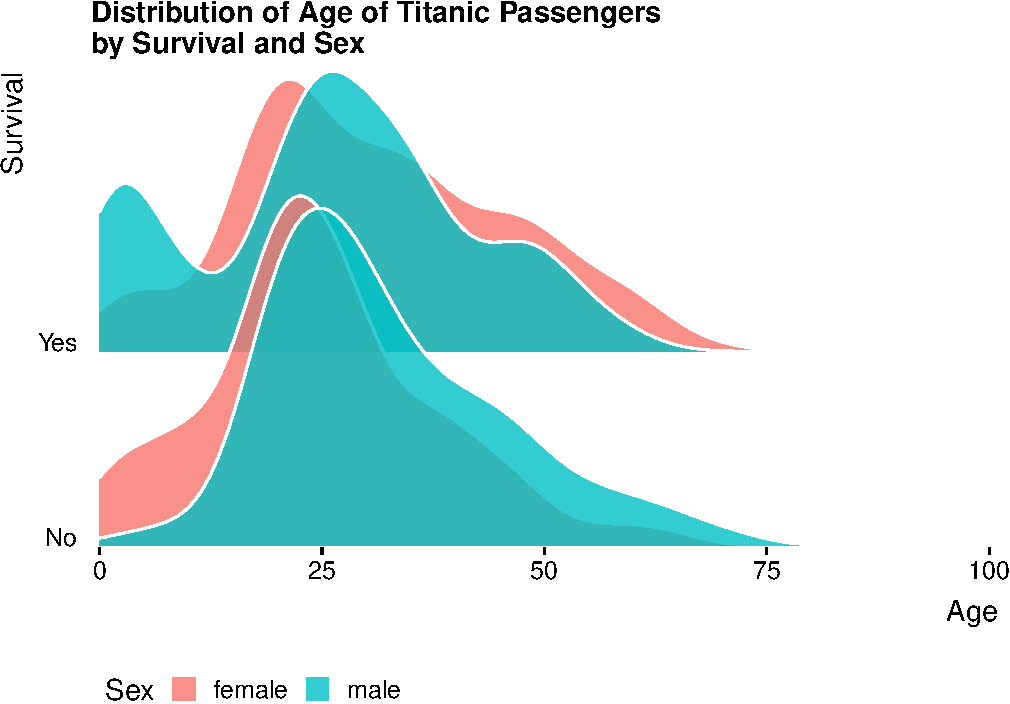
\includegraphics{Visualization_Examples_2020_v01_files/figure-latex/unnamed-chunk-3-1.pdf}

\hypertarget{quantitative-response-variable-and-categoricalbinary-explanatory-variable}{%
\subsection{Quantitative response variable and categorical/binary
explanatory
variable}\label{quantitative-response-variable-and-categoricalbinary-explanatory-variable}}

Remember that you could also use a boxplot for if you have a
quantitative response variable (let's say \texttt{age} just to keep the
Titanic data going). It's like the one above, but without flipping the y
and x axis.

\begin{Shaded}
\begin{Highlighting}[]
\NormalTok{PClass_Age_Box <-}\StringTok{ }\NormalTok{newTitanic }\OperatorTok\StringTok{ }\KeywordTok{ggplot}\NormalTok{(}\KeywordTok{aes}\NormalTok{(}\DataTypeTok{y =}\NormalTok{ Age, }\DataTypeTok{x =}\NormalTok{ PClass, }\DataTypeTok{fill =}\NormalTok{ Sex)) }\OperatorTok{+}\StringTok{ }
\StringTok{    }\KeywordTok{geom_boxplot}\NormalTok{(}\DataTypeTok{position =} \KeywordTok{position_dodge}\NormalTok{(}\FloatTok{0.9}\NormalTok{), }\DataTypeTok{lwd =} \FloatTok{1.2}\NormalTok{) }\OperatorTok{+}\StringTok{ }\KeywordTok{theme_bw}\NormalTok{() }\OperatorTok{+}\StringTok{ }
\StringTok{    }\KeywordTok{labs}\NormalTok{(}\DataTypeTok{y =} \StringTok{"Age"}\NormalTok{, }\DataTypeTok{x =} \StringTok{"Passenger Class"}\NormalTok{, }\DataTypeTok{title =} \StringTok{"Distribution of Age of Titanic Passengers }\CharTok{\textbackslash{}n}\StringTok{by Passenger Class and Sex"}\NormalTok{) }\OperatorTok{+}\StringTok{ }
\StringTok{    }\KeywordTok{theme}\NormalTok{(}\DataTypeTok{legend.position =} \StringTok{"bottom"}\NormalTok{, }\DataTypeTok{text =} \KeywordTok{element_text}\NormalTok{(}\DataTypeTok{size =} \DecValTok{20}\NormalTok{))}

\NormalTok{PClass_Age_Box}
\end{Highlighting}
\end{Shaded}

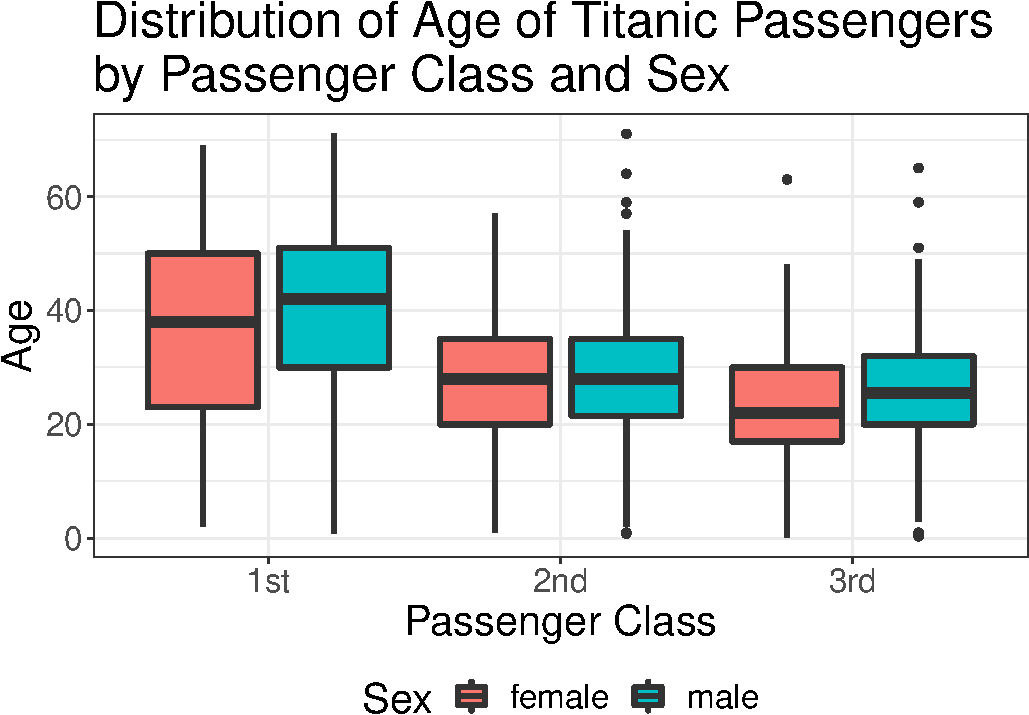
\includegraphics{Visualization_Examples_2020_v01_files/figure-latex/unnamed-chunk-4-1.pdf}

\hypertarget{binary-response-and-binary-explanatory-variables}{%
\subsection{Binary Response and Binary Explanatory
Variables}\label{binary-response-and-binary-explanatory-variables}}

\begin{Shaded}
\begin{Highlighting}[]
\CommentTok{# Here the explanatory variable is Sex and the response variable}
\CommentTok{# is Survived (yes/no) saving the plot as binary_by_binary,}
\CommentTok{# working from the Whickham data set}
\NormalTok{binary_by_binary <-}\StringTok{ }\NormalTok{Titanic }\OperatorTok\StringTok{ }\CommentTok{# by smoking status}
\KeywordTok{group_by}\NormalTok{(Sex) }\OperatorTok\StringTok{ }\CommentTok{# count how many are survived}
\KeywordTok{count}\NormalTok{(Survived) }\OperatorTok\StringTok{ }\CommentTok{# calculate the count as a proportion: (proprtion Survival of}
\CommentTok{# males; survival for females)}
\KeywordTok{mutate}\NormalTok{(}\DataTypeTok{pi =}\NormalTok{ n}\OperatorTok{/}\KeywordTok{sum}\NormalTok{(n)) }\OperatorTok\StringTok{ }\CommentTok{# only keep the survival outcomes (dead is just 1-pi)}
\KeywordTok{filter}\NormalTok{(Survived }\OperatorTok{==}\StringTok{ }\DecValTok{1}\NormalTok{) }\OperatorTok\StringTok{ }\CommentTok{# starting the plot of the probability of survival by sex}
\KeywordTok{ggplot}\NormalTok{(}\KeywordTok{aes}\NormalTok{(}\DataTypeTok{y =}\NormalTok{ pi, }\DataTypeTok{x =}\NormalTok{ Sex, }\DataTypeTok{fill =}\NormalTok{ Sex)) }\OperatorTok{+}\StringTok{ }\CommentTok{# Just naming the y-xis so it's clear which outcome we're plotting}
\CommentTok{# (alive or dead)}
\KeywordTok{ylab}\NormalTok{(}\StringTok{"Probabiltiy of Survival"}\NormalTok{) }\OperatorTok{+}\StringTok{ }\CommentTok{# plot the proportion/probability for Male and Female}
\KeywordTok{geom_bar}\NormalTok{(}\DataTypeTok{stat =} \StringTok{"identity"}\NormalTok{) }\OperatorTok{+}\StringTok{ }\KeywordTok{theme_bw}\NormalTok{() }\OperatorTok{+}\StringTok{ }\KeywordTok{theme}\NormalTok{(}\DataTypeTok{legend.position =} \StringTok{"bottom"}\NormalTok{)}

\NormalTok{binary_by_binary}
\end{Highlighting}
\end{Shaded}

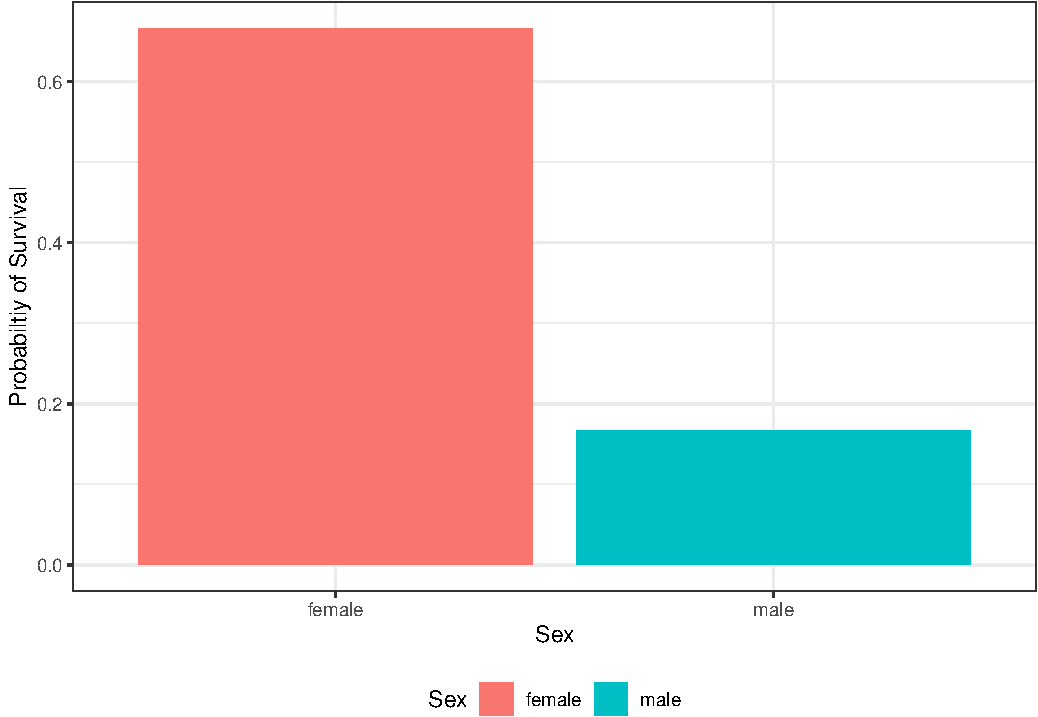
\includegraphics{Visualization_Examples_2020_v01_files/figure-latex/unnamed-chunk-5-1.pdf}

\hypertarget{visualizing-regression-models}{%
\section{Visualizing Regression
Models}\label{visualizing-regression-models}}

\begin{Shaded}
\begin{Highlighting}[]
\KeywordTok{library}\NormalTok{(tidyverse)}
\KeywordTok{library}\NormalTok{(Stat2Data)}
\KeywordTok{data}\NormalTok{(}\StringTok{"Titanic"}\NormalTok{)}
\end{Highlighting}
\end{Shaded}

\hypertarget{binary-repsonse-variables-logistic-regression-models}{%
\subsection{Binary Repsonse Variables / Logistic Regression
Models}\label{binary-repsonse-variables-logistic-regression-models}}

We're using the Titanic data to estimate the simple logistic regression
of differences in survival by sex (Model 1), and then a multiple
logistic regression model adjusted for age (Model 2).

\begin{Shaded}
\begin{Highlighting}[]
\NormalTok{model_}\DecValTok{1}\NormalTok{ <-}\StringTok{ }\KeywordTok{glm}\NormalTok{(Survived }\OperatorTok{~}\StringTok{ }\NormalTok{SexCode, }\DataTypeTok{family =}\NormalTok{ binomial, }\DataTypeTok{data =}\NormalTok{ Titanic)}
\NormalTok{model_}\DecValTok{2}\NormalTok{ <-}\StringTok{ }\KeywordTok{glm}\NormalTok{(Survived }\OperatorTok{~}\StringTok{ }\NormalTok{SexCode }\OperatorTok{+}\StringTok{ }\NormalTok{Age, }\DataTypeTok{family =}\NormalTok{ binomial, }\DataTypeTok{data =}\NormalTok{ Titanic)}
\end{Highlighting}
\end{Shaded}

Then we're going to use the \texttt{broom} package to exponentiate the
coefficients (i.e., calculating the OR), the confidence interval, and a
new variable to indicate which model it was from -- all saved into a
dataset. Once for each model, and then we're going to combine them
together into a new dataframe called oddsratios. And then we're going to
keep only the ORs and CIs for SexCode variable, since that's the only
one we want to illustrate -- this would likely be your main explanatory
variable from your main hypothesis that you want to depict across
multiple models.

\begin{Shaded}
\begin{Highlighting}[]
\KeywordTok{library}\NormalTok{(broom)}
\NormalTok{preds_}\DecValTok{1}\NormalTok{ <-}\StringTok{ }\KeywordTok{tidy}\NormalTok{(model_}\DecValTok{1}\NormalTok{, }\DataTypeTok{conf.int =} \OtherTok{TRUE}\NormalTok{, }\DataTypeTok{exponentiate =} \OtherTok{TRUE}\NormalTok{) }\OperatorTok\StringTok{ }
\StringTok{    }\KeywordTok{mutate}\NormalTok{(}\DataTypeTok{Model =} \StringTok{"Model 1"}\NormalTok{)}
\NormalTok{preds_}\DecValTok{2}\NormalTok{ <-}\StringTok{ }\KeywordTok{tidy}\NormalTok{(model_}\DecValTok{2}\NormalTok{, }\DataTypeTok{conf.int =} \OtherTok{TRUE}\NormalTok{, }\DataTypeTok{exponentiate =} \OtherTok{TRUE}\NormalTok{) }\OperatorTok\StringTok{ }
\StringTok{    }\KeywordTok{mutate}\NormalTok{(}\DataTypeTok{Model =} \StringTok{"Model 2"}\NormalTok{)}

\NormalTok{oddsratios <-}\StringTok{ }\KeywordTok{bind_rows}\NormalTok{(preds_}\DecValTok{1}\NormalTok{, preds_}\DecValTok{2}\NormalTok{)}
\NormalTok{oddsratios <-}\StringTok{ }\NormalTok{oddsratios }\OperatorTok\StringTok{ }\KeywordTok{filter}\NormalTok{(term }\OperatorTok\StringTok{ }\KeywordTok{c}\NormalTok{(}\StringTok{"SexCode"}\NormalTok{))}
\end{Highlighting}
\end{Shaded}

\hypertarget{plotting-the-odds-ratios}{%
\subsubsection{Plotting the Odds
Ratios}\label{plotting-the-odds-ratios}}

\begin{Shaded}
\begin{Highlighting}[]
\CommentTok{# Saving this as OR_plot, and working from the odds ratio dataset}
\NormalTok{OR_Plot<-}\StringTok{ }\NormalTok{oddsratios }\OperatorTok\StringTok{     }
\CommentTok{# Defining the Y as your estimated OR, x as the name of the OR }
\CommentTok{# (here, it's for SexCode) and coloring the Models differently}
\StringTok{  }\KeywordTok{ggplot}\NormalTok{(}\KeywordTok{aes}\NormalTok{(}\DataTypeTok{y =}\NormalTok{ estimate, }\DataTypeTok{x =}\NormalTok{ term, }\DataTypeTok{colour =}\NormalTok{ Model)) }\OperatorTok{+}
\StringTok{  }\CommentTok{# making the OR a point, with the CI as a line through the OR}
\StringTok{        }\KeywordTok{geom_pointrange}\NormalTok{(}\KeywordTok{aes}\NormalTok{(}\DataTypeTok{ymin =}\NormalTok{ conf.low, }\DataTypeTok{ymax =}\NormalTok{ conf.high),}
  \CommentTok{# dodged/offset horizontally to make it w}
                       \DataTypeTok{position =} \KeywordTok{position_dodge}\NormalTok{(}\DataTypeTok{width =} \FloatTok{0.5}\NormalTok{),          }
                       \DataTypeTok{size =} \FloatTok{.75}\NormalTok{) }\OperatorTok{+}
\StringTok{  }\CommentTok{# putting in a dotted line at the OR null = 1}
\StringTok{        }\KeywordTok{geom_hline}\NormalTok{(}\DataTypeTok{yintercept =} \FloatTok{1.0}\NormalTok{, }\DataTypeTok{linetype =} \StringTok{"dotted"}\NormalTok{, }\DataTypeTok{size =} \FloatTok{.5}\NormalTok{) }\OperatorTok{+}\StringTok{  }
\StringTok{  }\CommentTok{# Making the axis scale be on the log scale}
\StringTok{        }\KeywordTok{scale_y_log10}\NormalTok{(}\DataTypeTok{breaks =} \KeywordTok{c}\NormalTok{(}\DecValTok{0}\NormalTok{,}\FloatTok{0.5}\NormalTok{, }\FloatTok{1.0}\NormalTok{, }\DecValTok{2}\NormalTok{,}\DecValTok{5}\NormalTok{,}\DecValTok{10}\NormalTok{, }\DecValTok{15}\NormalTok{)) }\OperatorTok{+}\StringTok{   }
\StringTok{  }\CommentTok{# Labeling the x and y axes}
\StringTok{        }\KeywordTok{labs}\NormalTok{(}\DataTypeTok{y =} \StringTok{"Odds ratio"}\NormalTok{, }\DataTypeTok{x =} \StringTok{"Variable"}\NormalTok{) }\OperatorTok{+}\StringTok{   }
\StringTok{   }\CommentTok{# Flipping the y and x axes (similar to what we had to do with the boxplots)}
\StringTok{        }\KeywordTok{coord_flip}\NormalTok{(}\DataTypeTok{ylim =} \KeywordTok{c}\NormalTok{(}\FloatTok{0.5}\NormalTok{, }\DecValTok{16}\NormalTok{)) }\OperatorTok{+}\StringTok{ }
\StringTok{  }\CommentTok{# Making the background white instead of grey}
\StringTok{        }\KeywordTok{theme_bw}\NormalTok{()                                                      }
\NormalTok{OR_Plot}
\end{Highlighting}
\end{Shaded}

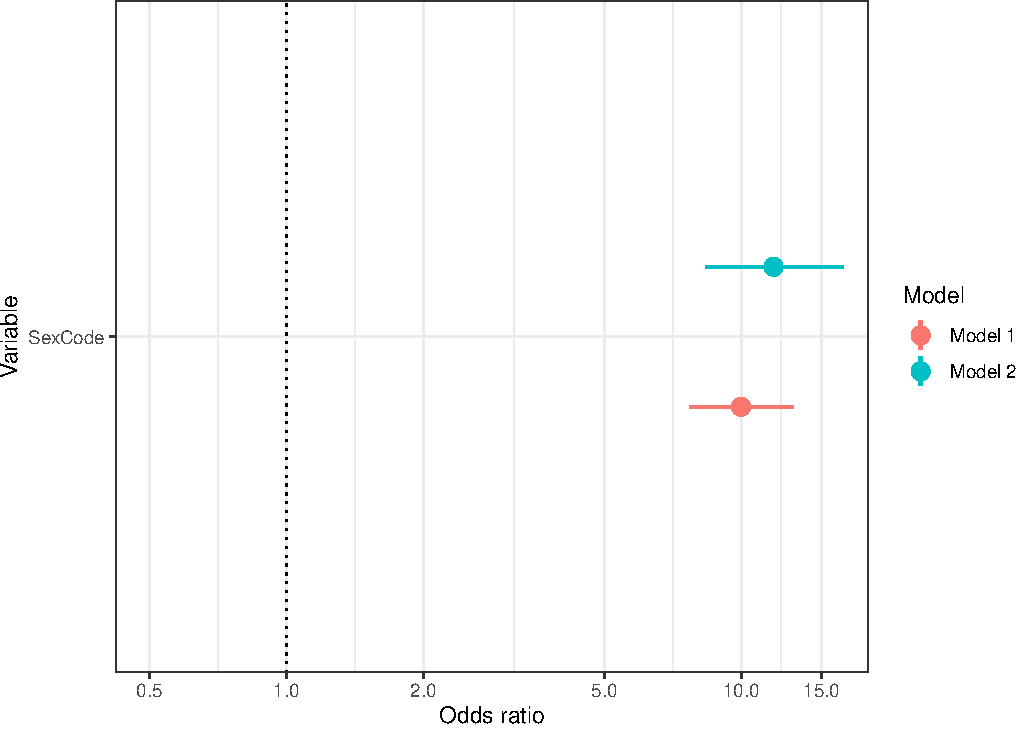
\includegraphics{Visualization_Examples_2020_v01_files/figure-latex/unnamed-chunk-9-1.pdf}

\begin{Shaded}
\begin{Highlighting}[]
\KeywordTok{ggsave}\NormalTok{(}\StringTok{"OR_plot.jpg"}\NormalTok{)}
\end{Highlighting}
\end{Shaded}

\begin{verbatim}
## Saving 7 x 5 in image
\end{verbatim}

For more insight and discussion of why you might want to depict the odds
ratio on the log scale, read a brief description
\href{https://academic.oup.com/aje/article/174/3/376/247288}{here.}
{[}note: this refers to ``risk'' which is similar to odds, and also
``relative odds'' which is a synonmym for ``odds ratio''{]}. The piece a
letter to the editor of the American Journal of Epidemiology, which, as
a journal, expects that any visual of ORs to be on the log scale. This
letter to the editor, from some former and current editors, explains
why.

\hypertarget{plotting-ors-for-categorical-explanatory-variable}{%
\paragraph{Plotting ORs for Categorical Explanatory
Variable}\label{plotting-ors-for-categorical-explanatory-variable}}

Now we're going to do a similar process but for a categorical
explanatory variable rather than binary: PClass as a simple logistic
regression model and then adjusted for Sex.

\begin{Shaded}
\begin{Highlighting}[]
\NormalTok{newTitanic <-}\StringTok{ }\NormalTok{Titanic }\OperatorTok\StringTok{ }\KeywordTok{filter}\NormalTok{(PClass }\OperatorTok{!=}\StringTok{ "*"}\NormalTok{)}
\NormalTok{PClass_}\DecValTok{1}\NormalTok{ <-}\StringTok{ }\KeywordTok{glm}\NormalTok{(Survived }\OperatorTok{~}\StringTok{ }\NormalTok{PClass, }\DataTypeTok{family =}\NormalTok{ binomial, }\DataTypeTok{data =}\NormalTok{ newTitanic)}
\NormalTok{PClass_preds_}\DecValTok{1}\NormalTok{ <-}\StringTok{ }\KeywordTok{tidy}\NormalTok{(PClass_}\DecValTok{1}\NormalTok{, }\DataTypeTok{conf.int =} \OtherTok{TRUE}\NormalTok{, }\DataTypeTok{exponentiate =} \OtherTok{TRUE}\NormalTok{) }\OperatorTok\StringTok{ }
\StringTok{    }\KeywordTok{mutate}\NormalTok{(}\DataTypeTok{Model =} \StringTok{"Unadjusted"}\NormalTok{)}

\NormalTok{PClass_}\DecValTok{2}\NormalTok{ <-}\StringTok{ }\KeywordTok{glm}\NormalTok{(Survived }\OperatorTok{~}\StringTok{ }\NormalTok{PClass }\OperatorTok{+}\StringTok{ }\NormalTok{SexCode, }\DataTypeTok{family =}\NormalTok{ binomial, }\DataTypeTok{data =}\NormalTok{ newTitanic)}
\NormalTok{PClass_preds_}\DecValTok{2}\NormalTok{ <-}\StringTok{ }\KeywordTok{tidy}\NormalTok{(PClass_}\DecValTok{2}\NormalTok{, }\DataTypeTok{conf.int =} \OtherTok{TRUE}\NormalTok{, }\DataTypeTok{exponentiate =} \OtherTok{TRUE}\NormalTok{) }\OperatorTok\StringTok{ }
\StringTok{    }\KeywordTok{mutate}\NormalTok{(}\DataTypeTok{Model =} \StringTok{"Sex Adjusted"}\NormalTok{)}

\NormalTok{PClass_OR <-}\StringTok{ }\KeywordTok{bind_rows}\NormalTok{(PClass_preds_}\DecValTok{1}\NormalTok{, PClass_preds_}\DecValTok{2}\NormalTok{)}
\NormalTok{PClass_OR <-}\StringTok{ }\NormalTok{PClass_OR }\OperatorTok\StringTok{ }\KeywordTok{filter}\NormalTok{(term }\OperatorTok\StringTok{ }\KeywordTok{c}\NormalTok{(}\StringTok{"PClass2nd"}\NormalTok{, }\StringTok{"PClass3rd"}\NormalTok{))}

\CommentTok{# Elements like pointrange and position_dodge only work when the}
\CommentTok{# outcome is mapped to y, need to go through with OR set as y then}
\CommentTok{# flip at the end}
\NormalTok{PClass_OR_plot <-}\StringTok{ }\NormalTok{PClass_OR }\OperatorTok\StringTok{ }\KeywordTok{ggplot}\NormalTok{(}\KeywordTok{aes}\NormalTok{(}\DataTypeTok{y =}\NormalTok{ estimate, }\DataTypeTok{x =}\NormalTok{ term, }
    \DataTypeTok{colour =}\NormalTok{ Model)) }\OperatorTok{+}\StringTok{ }\KeywordTok{geom_pointrange}\NormalTok{(}\KeywordTok{aes}\NormalTok{(}\DataTypeTok{ymin =}\NormalTok{ conf.low, }\DataTypeTok{ymax =}\NormalTok{ conf.high), }
    \DataTypeTok{position =} \KeywordTok{position_dodge}\NormalTok{(}\DataTypeTok{width =} \FloatTok{0.5}\NormalTok{), }\DataTypeTok{size =} \FloatTok{0.75}\NormalTok{) }\OperatorTok{+}\StringTok{ }\KeywordTok{geom_hline}\NormalTok{(}\DataTypeTok{yintercept =} \DecValTok{1}\NormalTok{, }
    \DataTypeTok{linetype =} \StringTok{"dotted"}\NormalTok{, }\DataTypeTok{size =} \FloatTok{0.5}\NormalTok{) }\OperatorTok{+}\StringTok{ }\KeywordTok{scale_y_log10}\NormalTok{(}\DataTypeTok{breaks =} \KeywordTok{c}\NormalTok{(}\DecValTok{0}\NormalTok{, }
    \FloatTok{0.1}\NormalTok{, }\FloatTok{0.25}\NormalTok{, }\FloatTok{0.5}\NormalTok{, }\DecValTok{1}\NormalTok{, }\FloatTok{1.5}\NormalTok{)) }\OperatorTok{+}\StringTok{ }\KeywordTok{labs}\NormalTok{(}\DataTypeTok{y =} \StringTok{"Odds ratio"}\NormalTok{, }\DataTypeTok{x =} \StringTok{"Variable"}\NormalTok{) }\OperatorTok{+}\StringTok{ }
\StringTok{    }\KeywordTok{coord_flip}\NormalTok{(}\DataTypeTok{ylim =} \KeywordTok{c}\NormalTok{(}\FloatTok{0.1}\NormalTok{, }\FloatTok{1.5}\NormalTok{)) }\OperatorTok{+}\StringTok{ }\KeywordTok{theme_bw}\NormalTok{()}

\NormalTok{PClass_OR_plot}
\end{Highlighting}
\end{Shaded}

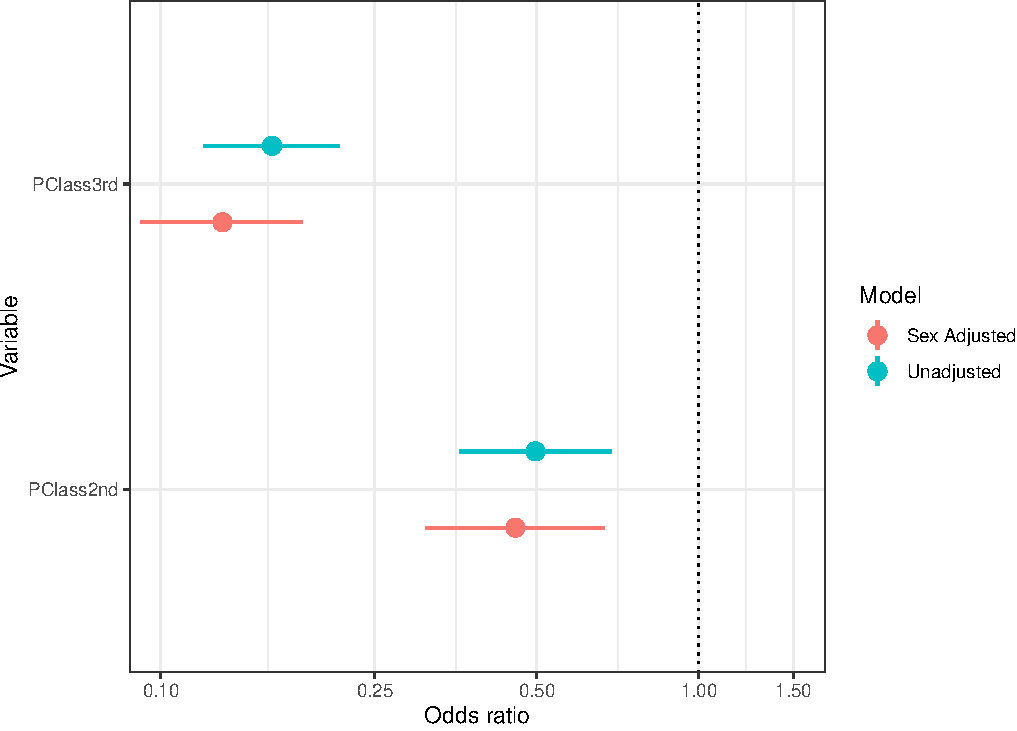
\includegraphics{Visualization_Examples_2020_v01_files/figure-latex/unnamed-chunk-10-1.pdf}

\begin{Shaded}
\begin{Highlighting}[]
\CommentTok{# This saves the figure, which is helpful for bringing into a}
\CommentTok{# poster or document.}
\KeywordTok{ggsave}\NormalTok{(}\StringTok{"PClass_OR_plot.jpg"}\NormalTok{)}
\end{Highlighting}
\end{Shaded}

\begin{verbatim}
## Saving 7 x 5 in image
\end{verbatim}

\hypertarget{predicted-probabilities}{%
\subsubsection{Predicted Probabilities}\label{predicted-probabilities}}

Maybe instead of odds ratios you want predicted probabilities - they're
more intuitive, etc. To do that, we're going to take slightly different
approach and use the \texttt{predict()} function like we have in
homeworks to get the predicted probability. Remember that the predict
function requires a ``new'' dataset with sample values for whom we want
the predicted probabilities to be calculated. We're going to use the
same model above: Survival as a function of PClass, adjusted for Sex.

\hypertarget{calculate-the-probabilities}{%
\paragraph{Calculate the
probabilities}\label{calculate-the-probabilities}}

First, we will generate a new dataset with the values of 1st, 2nd, and
3rd Class to apply to the PClass variable. We repeat it twice so that
there is a separate probability for men and women (this is similar to
what we did above with mean age, but there's no mean sex, so
illustrating both male and female probabilities makes more sense than
``holding sex constant at the mean''). These are saved in a newdataset
called ``newdat\_Titanic''

Then we predict the probability (type=``response'') of survival for men
and women in each passenger class from the regression coefficients
stored in PClass\_2. We also ask for the standard error (se.fit=TRUE) so
that we can calculate a confidence interval.

Lastly, we put those both together -- the sample data and the estimated
probability and standard error -- in a dataset called
\texttt{allpred\_Titanic}.

\begin{Shaded}
\begin{Highlighting}[]
\NormalTok{newdat_Titanic <-}\StringTok{ }\KeywordTok{data.frame}\NormalTok{(}\DataTypeTok{PClass =} \KeywordTok{c}\NormalTok{(}\StringTok{"1st"}\NormalTok{, }\StringTok{"2nd"}\NormalTok{, }\StringTok{"3rd"}\NormalTok{, }\StringTok{"1st"}\NormalTok{, }
    \StringTok{"2nd"}\NormalTok{, }\StringTok{"3rd"}\NormalTok{), }\DataTypeTok{SexCode =} \KeywordTok{c}\NormalTok{(}\DecValTok{0}\OperatorTok{:}\DecValTok{1}\NormalTok{))}
\NormalTok{pred_Titanic <-}\StringTok{ }\KeywordTok{as.data.frame}\NormalTok{(}\KeywordTok{predict}\NormalTok{(PClass_}\DecValTok{2}\NormalTok{, newdat_Titanic, }\DataTypeTok{se.fit =} \OtherTok{TRUE}\NormalTok{, }
    \DataTypeTok{type =} \StringTok{"response"}\NormalTok{))}
\NormalTok{allpred_Titanic <-}\StringTok{ }\KeywordTok{bind_cols}\NormalTok{(newdat_Titanic, pred_Titanic)}
\end{Highlighting}
\end{Shaded}

\hypertarget{plot-the-probabilities}{%
\paragraph{Plot the probabilities}\label{plot-the-probabilities}}

\begin{Shaded}
\begin{Highlighting}[]
\CommentTok{# Elements like pointrange and position_dodge only work when the outcome}
\CommentTok{#   is mapped to y, need to go through with OR set as y then flip at the}
\CommentTok{#   end}
\NormalTok{PClass_Prob_Plot <-}\StringTok{ }\NormalTok{allpred_Titanic }\OperatorTok
\StringTok{  }\KeywordTok{ggplot}\NormalTok{(}\KeywordTok{aes}\NormalTok{(}\DataTypeTok{y =}\NormalTok{ fit, }\DataTypeTok{x =}\NormalTok{ PClass, }\DataTypeTok{colour =} \KeywordTok{as.factor}\NormalTok{(SexCode))) }\OperatorTok{+}
\StringTok{        }\KeywordTok{geom_pointrange}\NormalTok{(}\KeywordTok{aes}\NormalTok{(}\DataTypeTok{ymin =}\NormalTok{ fit}\OperatorTok{-}\NormalTok{(}\FloatTok{1.96}\OperatorTok{*}\NormalTok{se.fit), }\DataTypeTok{ymax =}\NormalTok{ fit}\OperatorTok{+}\NormalTok{(}\FloatTok{1.96}\OperatorTok{*}\NormalTok{se.fit)),}
                       \DataTypeTok{position =} \KeywordTok{position_dodge}\NormalTok{(}\DataTypeTok{width =} \FloatTok{0.5}\NormalTok{),}
                       \DataTypeTok{size =} \FloatTok{.75}\NormalTok{) }\OperatorTok{+}
\StringTok{      }\CommentTok{# Legend label}
\StringTok{        }\KeywordTok{scale_color_hue}\NormalTok{(}\DataTypeTok{name=}\StringTok{"Sex"}\NormalTok{,             }
                      \CommentTok{# Defining the colors by your variable categories}
                     \DataTypeTok{breaks=}\KeywordTok{c}\NormalTok{(}\StringTok{"0"}\NormalTok{, }\StringTok{"1"}\NormalTok{), }
                     \CommentTok{# Making longer, sensible variable labels for the legend}
                     \DataTypeTok{labels=}\KeywordTok{c}\NormalTok{(}\StringTok{"Male"}\NormalTok{,   }
                       \StringTok{"Female"}\NormalTok{)) }\OperatorTok{+}
\StringTok{       }\CommentTok{# geom_hline(yintercept = 1.0, linetype = "dotted", size = .5) +}
\StringTok{        }\CommentTok{#scale_y_log10(breaks = c(0,0.1,0.25,0.5, 1.0, 1.5)) +}
\StringTok{        }\KeywordTok{labs}\NormalTok{(}\DataTypeTok{y =} \StringTok{"Probability of Survival"}\NormalTok{, }\DataTypeTok{x =} \StringTok{"Passenger Class"}\NormalTok{) }\OperatorTok{+}
\StringTok{        }\CommentTok{#coord_flip(ylim = c(0.1, 1.5)) +}
\StringTok{        }\KeywordTok{theme_bw}\NormalTok{()}
\NormalTok{PClass_Prob_Plot}
\end{Highlighting}
\end{Shaded}

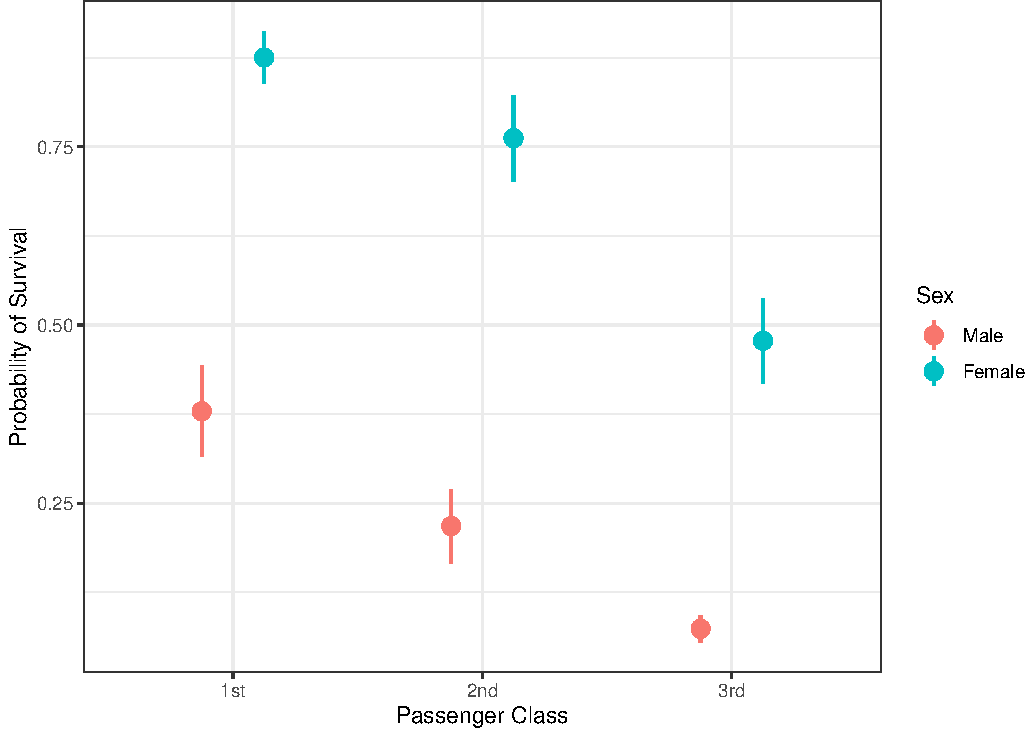
\includegraphics{Visualization_Examples_2020_v01_files/figure-latex/unnamed-chunk-12-1.pdf}

\begin{Shaded}
\begin{Highlighting}[]
\KeywordTok{ggsave}\NormalTok{(}\StringTok{"PClass_Prob_Plot.jpg"}\NormalTok{)}
\end{Highlighting}
\end{Shaded}

\begin{verbatim}
## Saving 7 x 5 in image
\end{verbatim}

\hypertarget{binary-explanatory-and-quantitative-response}{%
\subsection{Binary Explanatory and Quantitative
Response}\label{binary-explanatory-and-quantitative-response}}

Similar to what we did above with the predicted probability, if you have
a quantiative response variable, we can do a similar process to estimate
the predicted value (\(\hat{y}\)) of the response variable for binary
explanatory variables. (If you have quantitative explanatory variables,
you could use the example code from the travel time example and show a
linear slope for that quantitative variable).

Here, the data are an extension of our original PorschePrice example --
now with 2 car types: Porsche or Jaguars -- used to predict the price of
a used car. I am also including another binary variable -- how old the
used car is -- to mimic a binary*binary interaction that some groups are
having.

First I'm creating those variables, and estimating a model of
\(y = \beta_0+\beta_1 Type + \beta_2 Age + \beta_3 Type*Age + \beta_4 Mileage + \epsilon\)
Then I'm calculating the mean number of miles to predict the estimated
price of the car for by type and age of the average number of miles.
You'll want / need to do this for your confounding variables.

Then we're doing a very similar process as above (see that section for
details) with the predict function. Here we're able to calculate the
confidence interval around that prediction directly.

\begin{Shaded}
\begin{Highlighting}[]
\KeywordTok{data}\NormalTok{(}\StringTok{"PorscheJaguar"}\NormalTok{)}
\NormalTok{PJ <-}\StringTok{ }\NormalTok{PorscheJaguar }\OperatorTok\StringTok{ }\KeywordTok{mutate}\NormalTok{(}\DataTypeTok{age_le5 =} \KeywordTok{as.factor}\NormalTok{(}\KeywordTok{if_else}\NormalTok{(Age }\OperatorTok{<}\StringTok{ }\DecValTok{5}\NormalTok{, }
    \StringTok{"< 5yo"}\NormalTok{, }\KeywordTok{if_else}\NormalTok{(Age }\OperatorTok{>=}\StringTok{ }\DecValTok{5}\NormalTok{, }\StringTok{"5+yo"}\NormalTok{, }\OtherTok{NA_character_}\NormalTok{))))}

\NormalTok{m0 <-}\StringTok{ }\KeywordTok{lm}\NormalTok{(Price }\OperatorTok{~}\StringTok{ }\NormalTok{Car }\OperatorTok{*}\StringTok{ }\NormalTok{age_le5 }\OperatorTok{+}\StringTok{ }\NormalTok{Mileage, }\DataTypeTok{data =}\NormalTok{ PJ)}
\KeywordTok{summary}\NormalTok{(m0)}
\end{Highlighting}
\end{Shaded}

\begin{verbatim}
## 
## Call:
## lm(formula = Price ~ Car * age_le5 + Mileage, data = PJ)
## 
## Residuals:
##      Min       1Q   Median       3Q      Max 
## -21.3237  -5.3639  -0.6174   5.3603  18.8844 
## 
## Coefficients:
##                        Estimate Std. Error t value Pr(>|t|)    
## (Intercept)            54.75720    2.85205  19.199  < 2e-16 ***
## CarPorsche             15.60613    3.22845   4.834 1.12e-05 ***
## age_le55+yo            -8.43185    3.71450  -2.270   0.0271 *  
## Mileage                -0.50197    0.06816  -7.365 9.53e-10 ***
## CarPorsche:age_le55+yo  2.62758    4.65649   0.564   0.5749    
## ---
## Signif. codes:  0 '***' 0.001 '**' 0.01 '*' 0.05 '.' 0.1 ' ' 1
## 
## Residual standard error: 8.866 on 55 degrees of freedom
## Multiple R-squared:  0.7877, Adjusted R-squared:  0.7723 
## F-statistic: 51.03 on 4 and 55 DF,  p-value: < 2.2e-16
\end{verbatim}

\begin{Shaded}
\begin{Highlighting}[]
\NormalTok{meanMiles <-}\StringTok{ }\KeywordTok{mean}\NormalTok{(PJ}\OperatorTok{$}\NormalTok{Mileage)}
\NormalTok{newdat <-}\StringTok{ }\KeywordTok{data.frame}\NormalTok{(}\DataTypeTok{Car =} \KeywordTok{c}\NormalTok{(}\StringTok{"Porsche"}\NormalTok{, }\StringTok{"Porsche"}\NormalTok{, }\StringTok{"Jaguar"}\NormalTok{, }\StringTok{"Jaguar"}\NormalTok{), }
    \DataTypeTok{age_le5 =} \KeywordTok{c}\NormalTok{(}\StringTok{"< 5yo"}\NormalTok{, }\StringTok{"5+yo"}\NormalTok{), }\DataTypeTok{Mileage =}\NormalTok{ meanMiles)}
\NormalTok{preds <-}\StringTok{ }\KeywordTok{as.data.frame}\NormalTok{(}\KeywordTok{predict}\NormalTok{(m0, newdat, }\DataTypeTok{interval =} \StringTok{"confidence"}\NormalTok{, }
    \DataTypeTok{level =} \FloatTok{0.95}\NormalTok{))}
\NormalTok{allpreds <-}\StringTok{ }\KeywordTok{bind_cols}\NormalTok{(newdat, preds)}
\end{Highlighting}
\end{Shaded}

\hypertarget{plotting}{%
\subsubsection{Plotting}\label{plotting}}

\hypertarget{with-a-point-and-ci-for-the-prediction-around-the-point}{%
\paragraph{With a point and CI for the prediction around the
point}\label{with-a-point-and-ci-for-the-prediction-around-the-point}}

\begin{Shaded}
\begin{Highlighting}[]
\NormalTok{Price_point<-allpreds }\OperatorTok\StringTok{ }\KeywordTok{ggplot}\NormalTok{(}\KeywordTok{aes}\NormalTok{(}\DataTypeTok{x=}\NormalTok{Car, }\DataTypeTok{y=}\NormalTok{fit, }
                                     \DataTypeTok{colour=}\NormalTok{age_le5, }\DataTypeTok{group=}\NormalTok{age_le5)) }\OperatorTok{+}\StringTok{ }
\StringTok{    }\KeywordTok{geom_errorbar}\NormalTok{(}\KeywordTok{aes}\NormalTok{(}\DataTypeTok{ymin=}\NormalTok{lwr, }\DataTypeTok{ymax=}\NormalTok{upr), }
 \CommentTok{# Defining }
      \DataTypeTok{width=}\NormalTok{.}\DecValTok{1}\NormalTok{, }\DataTypeTok{position=}\KeywordTok{position_dodge}\NormalTok{(}\FloatTok{0.1}\NormalTok{)) }\OperatorTok{+}
\StringTok{  }\CommentTok{# Slightly offsetting the points by group}
\StringTok{    }\KeywordTok{geom_point}\NormalTok{(}\DataTypeTok{position=}\KeywordTok{position_dodge}\NormalTok{(}\FloatTok{0.1}\NormalTok{),}
  \CommentTok{# Making the points smaller}
      \DataTypeTok{size=}\DecValTok{3}\NormalTok{) }\OperatorTok{+}\StringTok{ }
\StringTok{    }\CommentTok{# Changing x-axis label}
\StringTok{    }\KeywordTok{xlab}\NormalTok{(}\StringTok{"Car Make"}\NormalTok{) }\OperatorTok{+}\StringTok{ }
\StringTok{   }\CommentTok{# Changing y-axis label}
\StringTok{    }\KeywordTok{ylab}\NormalTok{(}\StringTok{"Estimated Price (in $1,000s)"}\NormalTok{) }\OperatorTok{+}
\StringTok{  }\CommentTok{# Legend label}
\StringTok{    }\KeywordTok{scale_color_hue}\NormalTok{(}\DataTypeTok{name=}\StringTok{"Car Age"}\NormalTok{,}
  \CommentTok{# Defining the colors by your variable categories                  }
                     \DataTypeTok{breaks=}\KeywordTok{c}\NormalTok{(}\StringTok{"< 5yo"}\NormalTok{, }\StringTok{"5+yo"}\NormalTok{), }
   \CommentTok{# Making longer, sensible variable labels for the legend}
                     \DataTypeTok{labels=}\KeywordTok{c}\NormalTok{(}\StringTok{"<5 years old"}\NormalTok{,  }
                       \StringTok{"5+ years old"}\NormalTok{)) }\OperatorTok{+}
\StringTok{  }\CommentTok{# Title for the overall graph}
\StringTok{    }\KeywordTok{ggtitle}\NormalTok{(}\StringTok{"Predicted Price of Used Car by Make and Age, adjusted for Mileage"}\NormalTok{) }\OperatorTok{+}\StringTok{ }
\StringTok{  }\CommentTok{# Expand y range to start at 0}
\StringTok{    }\KeywordTok{expand_limits}\NormalTok{(}\DataTypeTok{y=}\DecValTok{0}\NormalTok{) }\OperatorTok{+}\StringTok{           }
\StringTok{  }\CommentTok{# Set tick every 5}
\StringTok{    }\KeywordTok{scale_y_continuous}\NormalTok{(}\DataTypeTok{breaks=}\DecValTok{0}\OperatorTok{:}\DecValTok{60}\OperatorTok{*}\DecValTok{10}\NormalTok{) }\OperatorTok{+}\StringTok{ }
\StringTok{   }\CommentTok{# Making }
\StringTok{    }\KeywordTok{theme_bw}\NormalTok{() }\OperatorTok{+}\StringTok{                     }
\StringTok{  }\CommentTok{# Position legend in bottom centered}
\StringTok{    }\KeywordTok{theme}\NormalTok{(}\DataTypeTok{legend.position=}\StringTok{"bottom"}\NormalTok{)             }

\NormalTok{Price_point}
\end{Highlighting}
\end{Shaded}

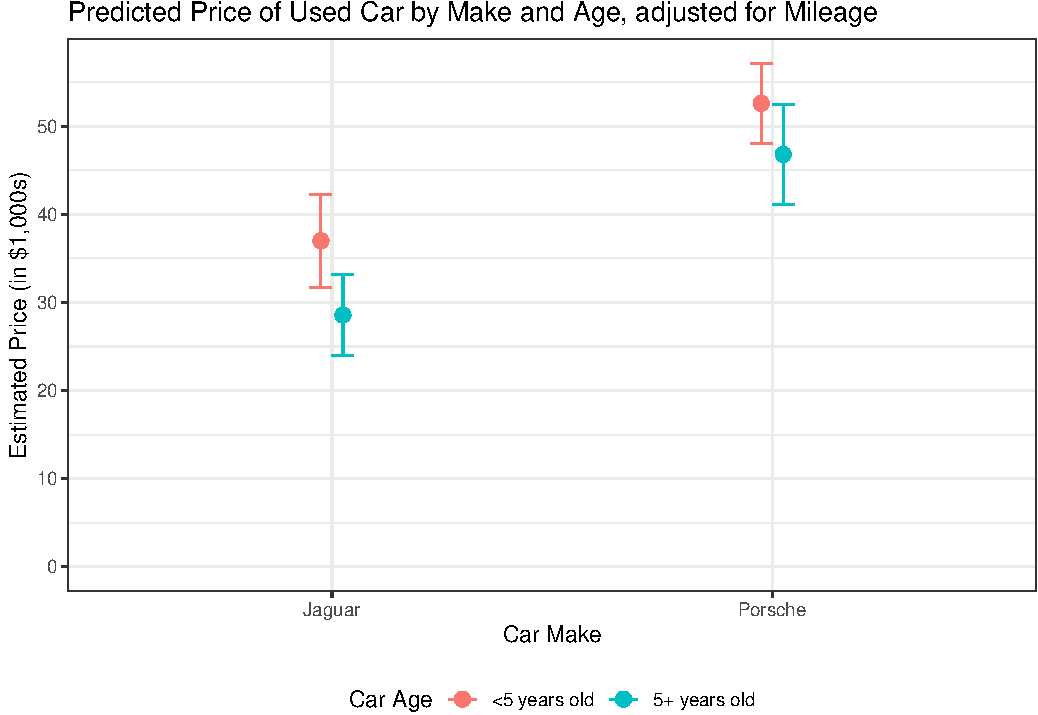
\includegraphics{Visualization_Examples_2020_v01_files/figure-latex/unnamed-chunk-14-1.pdf}

\begin{Shaded}
\begin{Highlighting}[]
\KeywordTok{ggsave}\NormalTok{(}\StringTok{"Price_point.jpg"}\NormalTok{)}
\end{Highlighting}
\end{Shaded}

\begin{verbatim}
## Saving 7 x 5 in image
\end{verbatim}

\hypertarget{same-as-above-but-as-a-bar}{%
\paragraph{Same as above but as a
bar}\label{same-as-above-but-as-a-bar}}

Here the top of the bar is the predicted price. It's a little goofy to
depict as a bar, but you could imagine that the bar height is literally
the stack of \$1 bills for the price of that car.

\begin{Shaded}
\begin{Highlighting}[]
\NormalTok{Price_bar<-allpreds }\OperatorTok\StringTok{ }
\StringTok{  }\KeywordTok{ggplot}\NormalTok{(}
\CommentTok{# Defining x, y axis and }
\CommentTok{# the grouping variable that fills in the bar}
  \KeywordTok{aes}\NormalTok{(}\DataTypeTok{x=}\NormalTok{Car, }\DataTypeTok{y=}\NormalTok{fit, }\DataTypeTok{fill=}\NormalTok{age_le5)) }\OperatorTok{+}
\CommentTok{# Dodge makes the bars be next to each other}
\StringTok{    }\KeywordTok{geom_bar}\NormalTok{(}\DataTypeTok{position=}\KeywordTok{position_dodge}\NormalTok{(.}\DecValTok{9}\NormalTok{),}
\CommentTok{# Making the bars}
      \DataTypeTok{stat=}\StringTok{"identity"}\NormalTok{) }\OperatorTok{+}\StringTok{                       }
\StringTok{    }\KeywordTok{geom_errorbar}\NormalTok{(}\DataTypeTok{position=}\KeywordTok{position_dodge}\NormalTok{(.}\DecValTok{9}\NormalTok{),}
\CommentTok{# Defining the CI levels and line width}
      \DataTypeTok{width=}\NormalTok{.}\DecValTok{25}\NormalTok{, }\KeywordTok{aes}\NormalTok{(}\DataTypeTok{ymin=}\NormalTok{lwr, }\DataTypeTok{ymax=}\NormalTok{upr)) }\OperatorTok{+}
\CommentTok{# Changing x-axis label}
\StringTok{    }\KeywordTok{xlab}\NormalTok{(}\StringTok{"Car Make"}\NormalTok{) }\OperatorTok{+}
\StringTok{ }\CommentTok{# Changing y-axis label}
\StringTok{    }\KeywordTok{ylab}\NormalTok{(}\StringTok{"Estimated Price (in $1,000s)"}\NormalTok{) }\OperatorTok{+}
\StringTok{ }\CommentTok{# Legend label}
\StringTok{    }\KeywordTok{scale_fill_discrete}\NormalTok{(}\DataTypeTok{name=}\StringTok{"Car Age"}\NormalTok{,}
\CommentTok{# Defining the colors by your variable categories}
                     \DataTypeTok{breaks=}\KeywordTok{c}\NormalTok{(}\StringTok{"< 5yo"}\NormalTok{, }\StringTok{"5+yo"}\NormalTok{),}
\CommentTok{# Making longer, sensible variable labels for the legend}
                     \DataTypeTok{labels=}\KeywordTok{c}\NormalTok{(}\StringTok{"<5 years old"}\NormalTok{,   }
                       \StringTok{"5+ years old"}\NormalTok{)) }\OperatorTok{+}
\StringTok{  }\CommentTok{# Title for the overall graph}
\StringTok{    }\KeywordTok{ggtitle}\NormalTok{(}\StringTok{"Predicted Price of Used Car by Make and Age, adjusted for Mileage"}\NormalTok{) }\OperatorTok{+}
\StringTok{  }\CommentTok{# Expand y range to start at 0}
\StringTok{    }\KeywordTok{expand_limits}\NormalTok{(}\DataTypeTok{y=}\DecValTok{0}\NormalTok{) }\OperatorTok{+}\StringTok{ }
\StringTok{  }\CommentTok{# Set tick every 5}
\StringTok{    }\KeywordTok{scale_y_continuous}\NormalTok{(}\DataTypeTok{breaks=}\DecValTok{0}\OperatorTok{:}\DecValTok{60}\OperatorTok{*}\DecValTok{10}\NormalTok{) }\OperatorTok{+}
\StringTok{   }\CommentTok{# Making the grey background go away}
\StringTok{    }\KeywordTok{theme_bw}\NormalTok{() }\OperatorTok{+}\StringTok{                   }
\StringTok{  }\CommentTok{# Position legend in bottom centered}
\StringTok{    }\KeywordTok{theme}\NormalTok{(}\DataTypeTok{legend.position=}\StringTok{"bottom"}\NormalTok{)}

\NormalTok{Price_bar}
\end{Highlighting}
\end{Shaded}

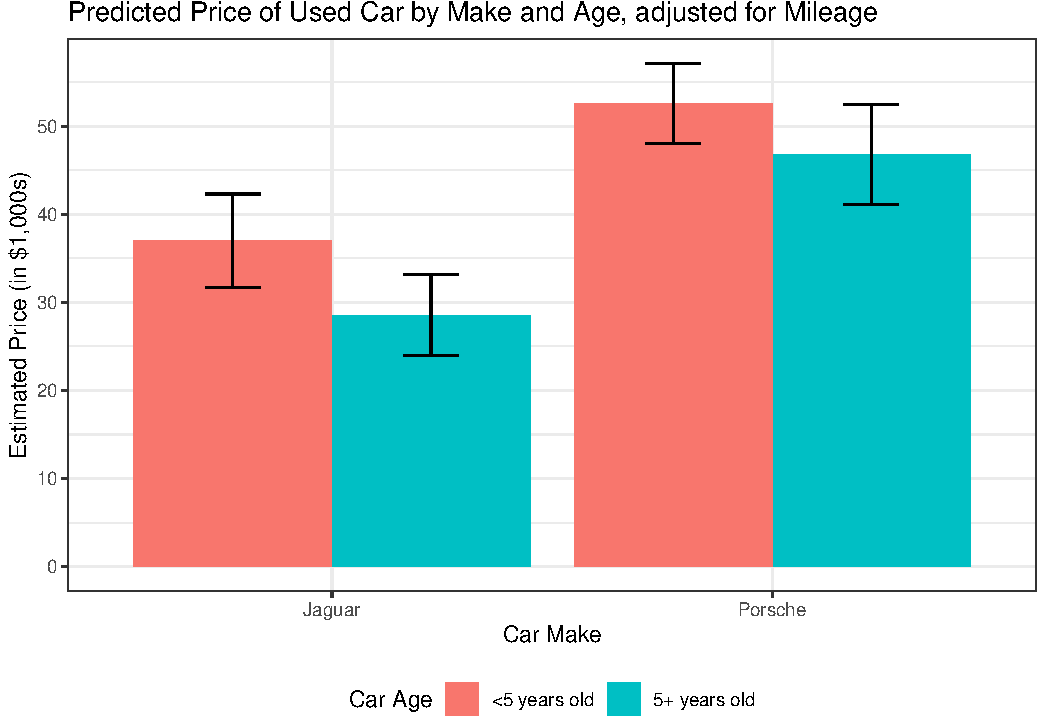
\includegraphics{Visualization_Examples_2020_v01_files/figure-latex/unnamed-chunk-15-1.pdf}

\begin{Shaded}
\begin{Highlighting}[]
\KeywordTok{ggsave}\NormalTok{(}\StringTok{"Price_bar.jpg"}\NormalTok{)}
\end{Highlighting}
\end{Shaded}

\begin{verbatim}
## Saving 7 x 5 in image
\end{verbatim}

\end{document}
